%%%%%%%%%%%%%%%%%%%% Platform Model %%%%%%%%%%%%%%%%%%%%%%

% \begin{frame}{OpenCL Platform Model}
%  \begin{center}
%    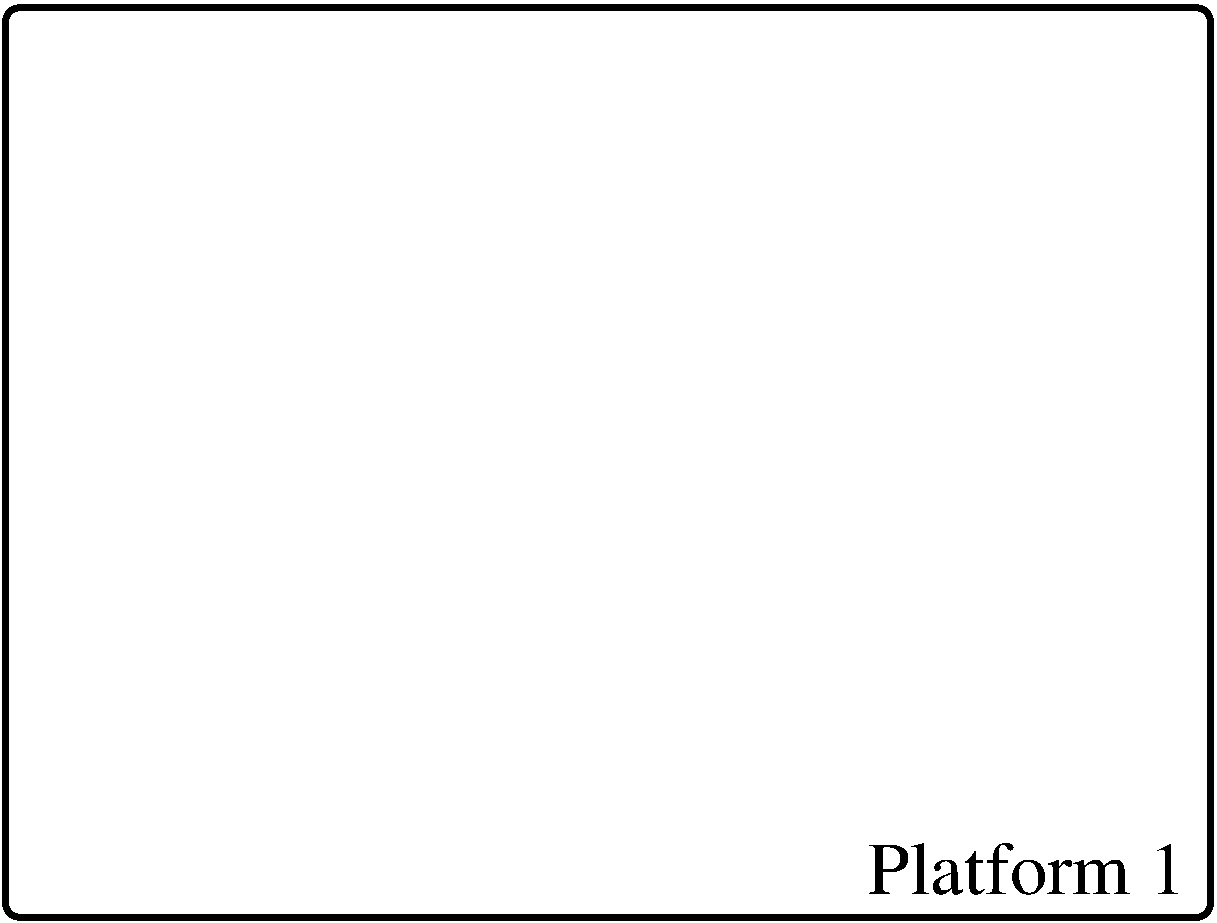
\includegraphics[width=0.80\textwidth]{figures/opencl-2.pdf}
%  \end{center}
% \end{frame}
% 
% \begin{frame}{OpenCL Platform Model}
%  \begin{center}
%    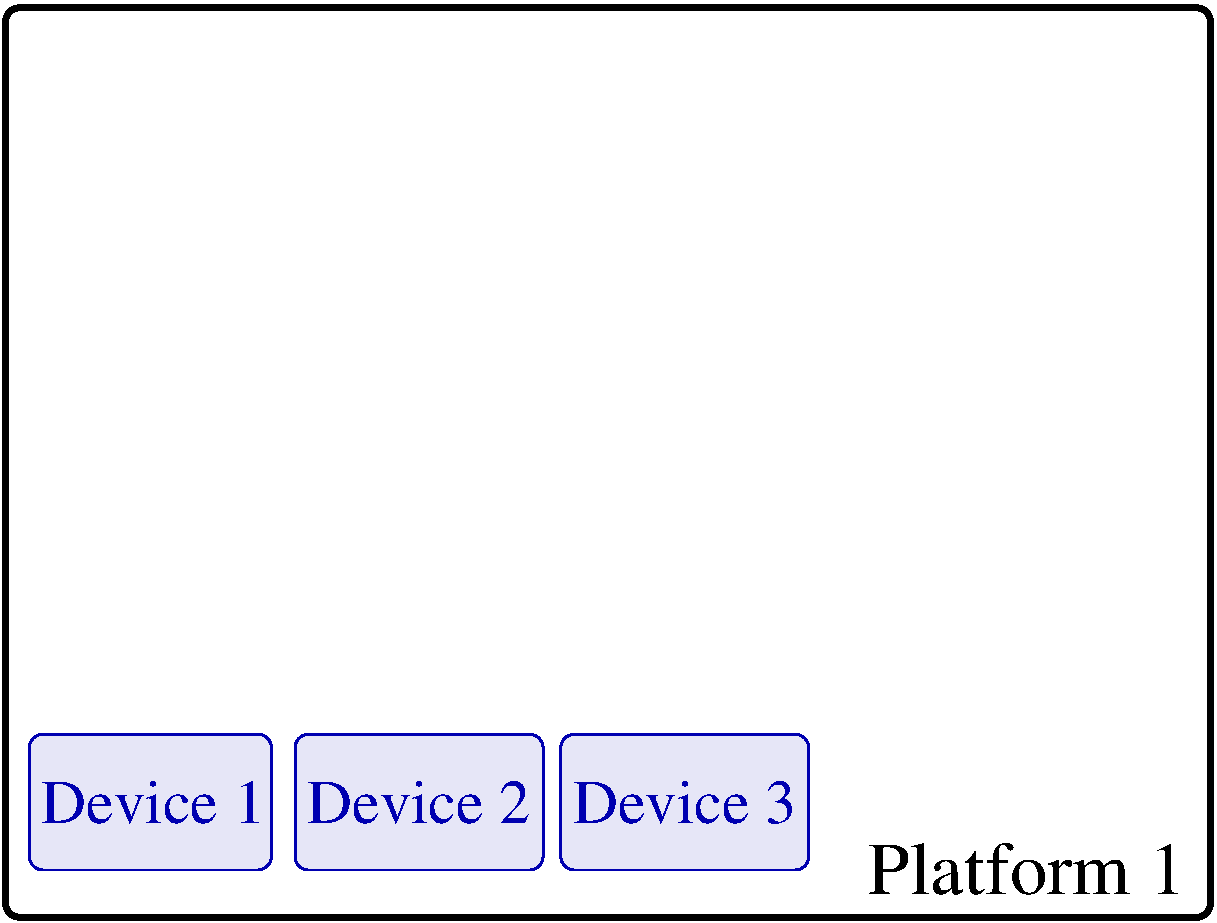
\includegraphics[width=0.80\textwidth]{figures/opencl-3.pdf}
%  \end{center}
% \end{frame}
% 
% \begin{frame}{OpenCL Platform Model}
%  \begin{center}
%    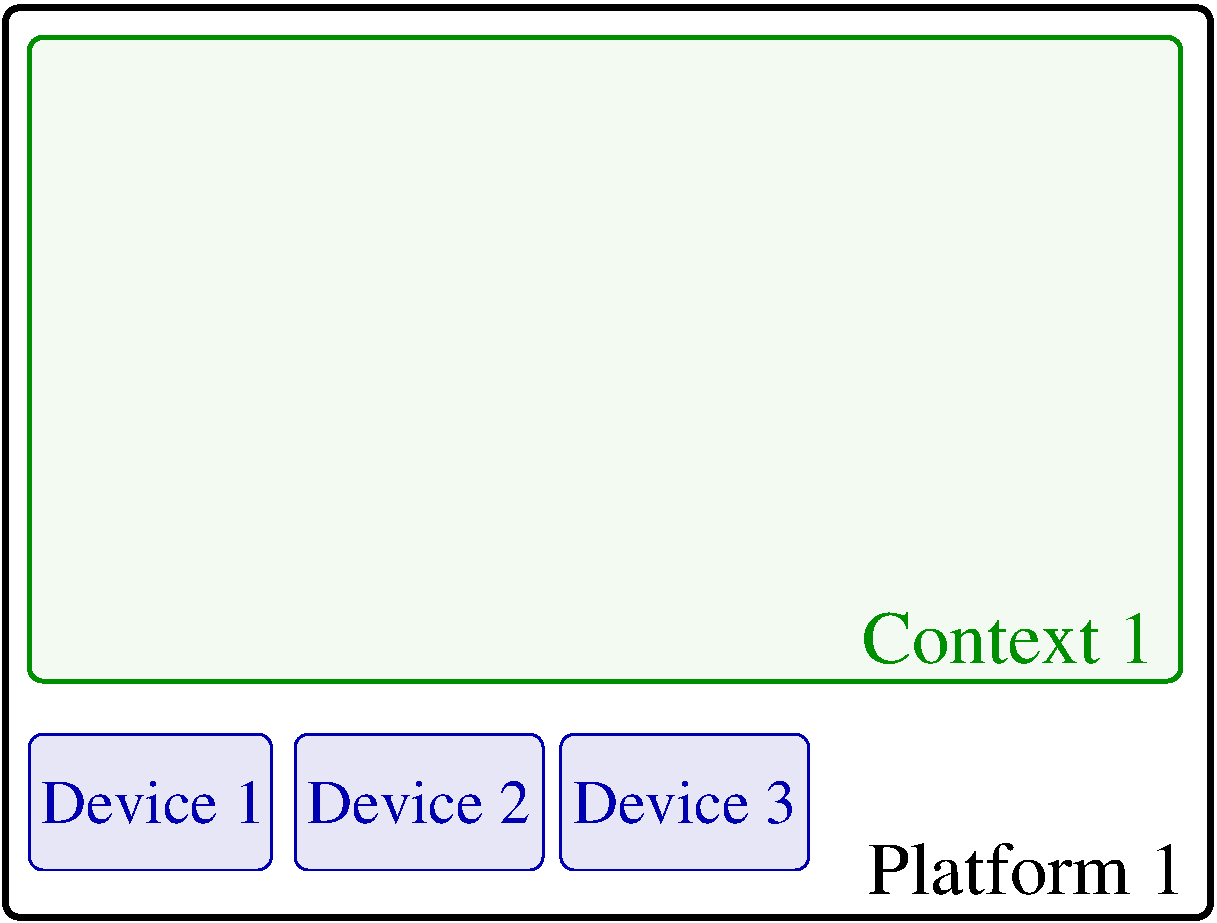
\includegraphics[width=0.80\textwidth]{figures/opencl-4.pdf}
%  \end{center}
% \end{frame}
% 
% \begin{frame}{OpenCL Platform Model}
%  \begin{center}
%    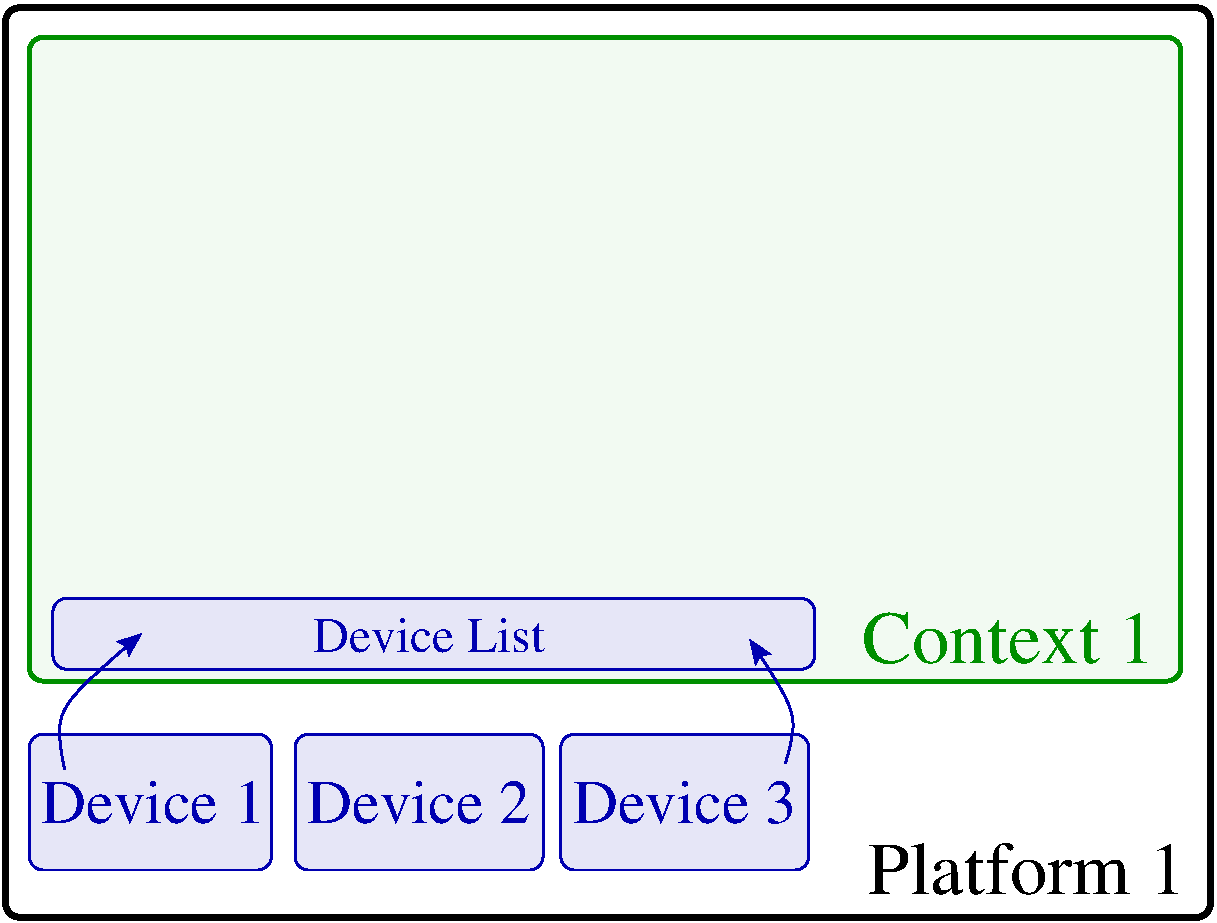
\includegraphics[width=0.80\textwidth]{figures/opencl-5.pdf}
%  \end{center}
% \end{frame}
% 
% \begin{frame}{OpenCL Platform Model}
%  \begin{center}
%    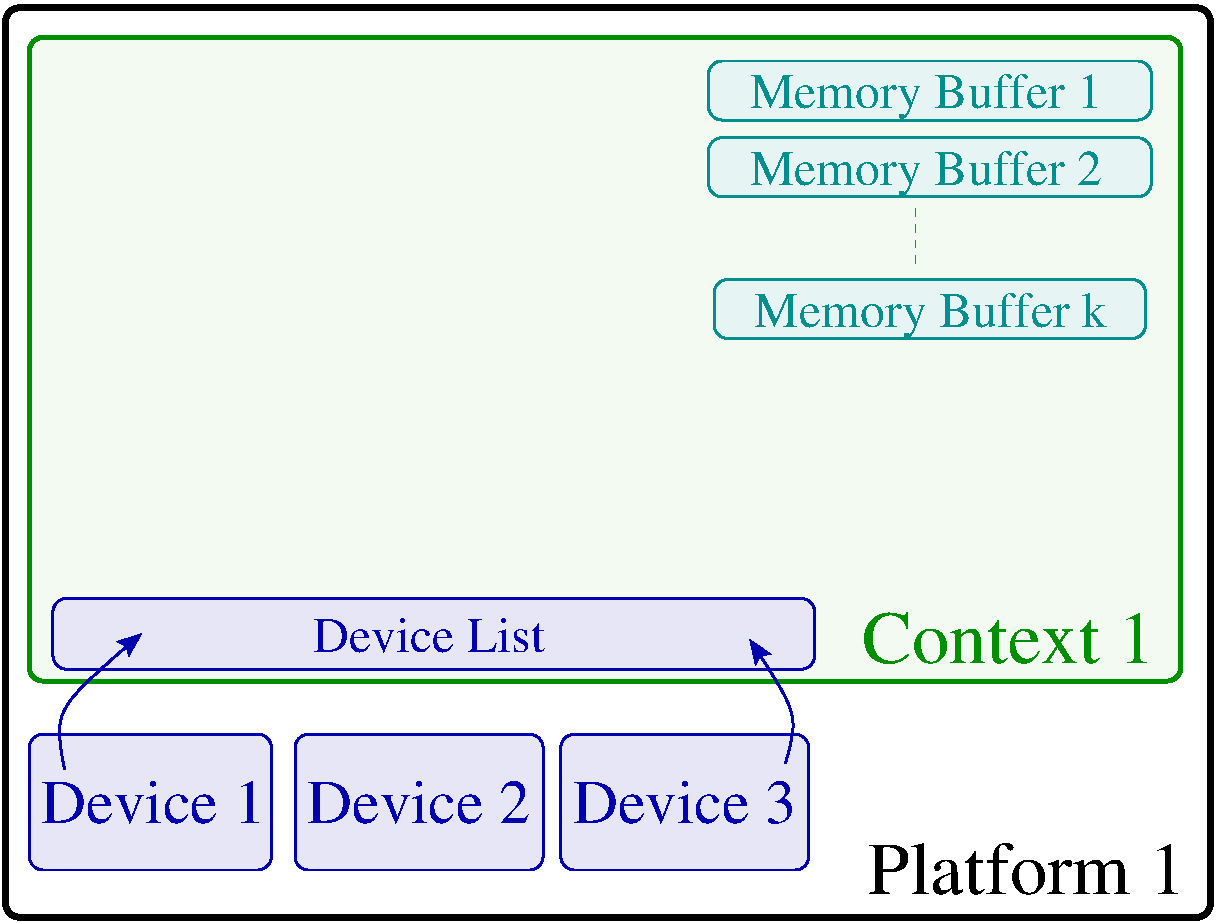
\includegraphics[width=0.80\textwidth]{figures/opencl-6.pdf}
%  \end{center}
% \end{frame}
% 
% \begin{frame}{OpenCL Platform Model}
%  \begin{center}
%    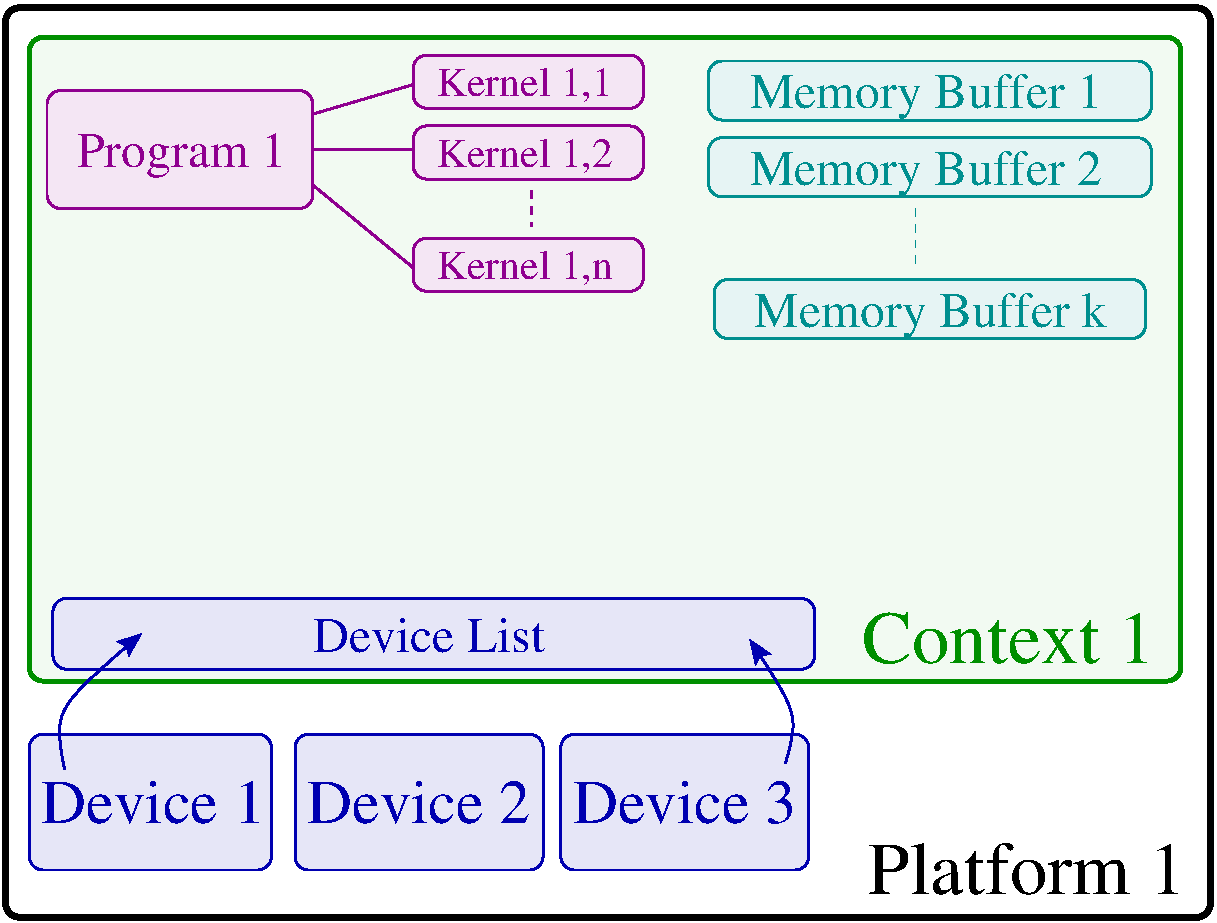
\includegraphics[width=0.80\textwidth]{figures/opencl-7.pdf}
%  \end{center}
% \end{frame}
% 
% \begin{frame}{OpenCL Platform Model}
%  \begin{center}
%    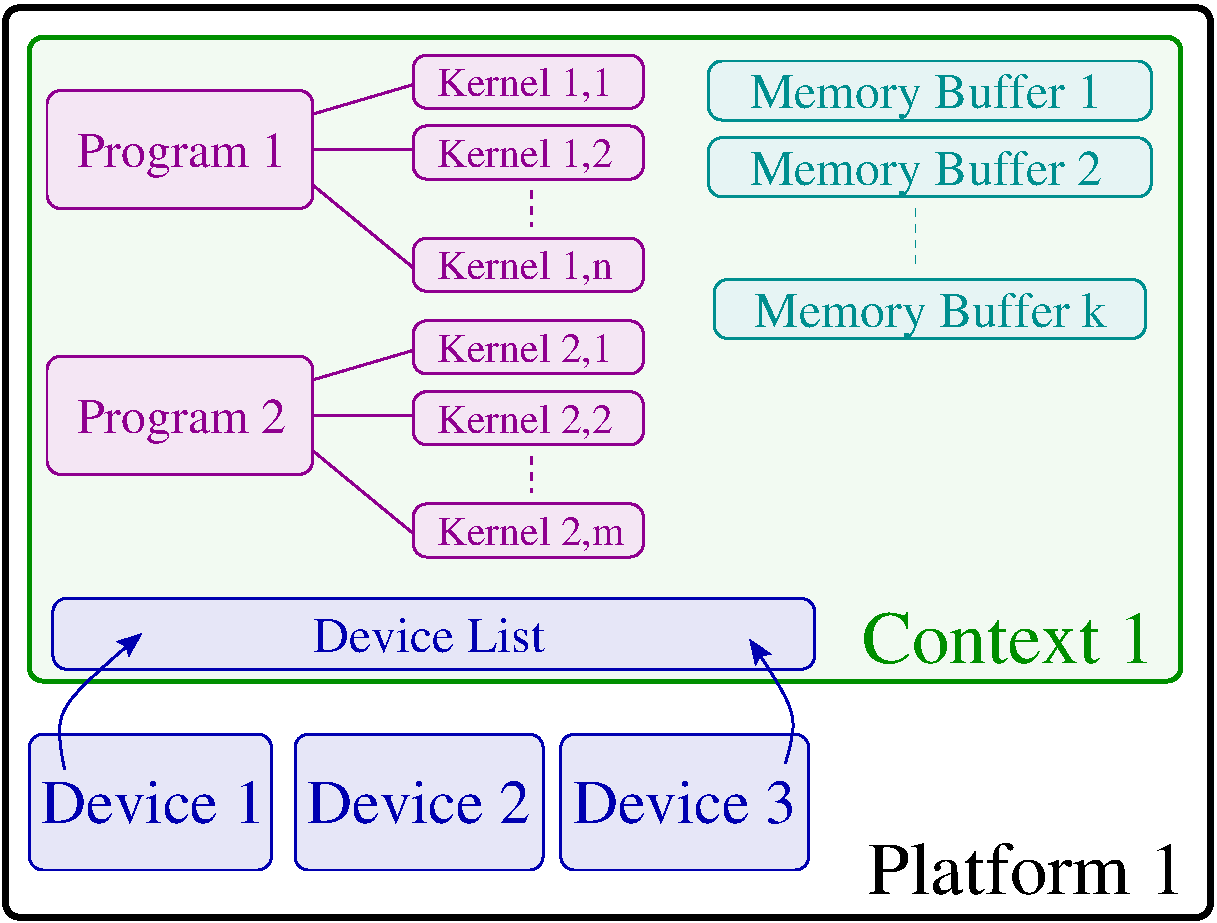
\includegraphics[width=0.80\textwidth]{figures/opencl-8.pdf}
%  \end{center}
% \end{frame}

\begin{frame}{OpenCL Platform Model}
 \begin{center}
   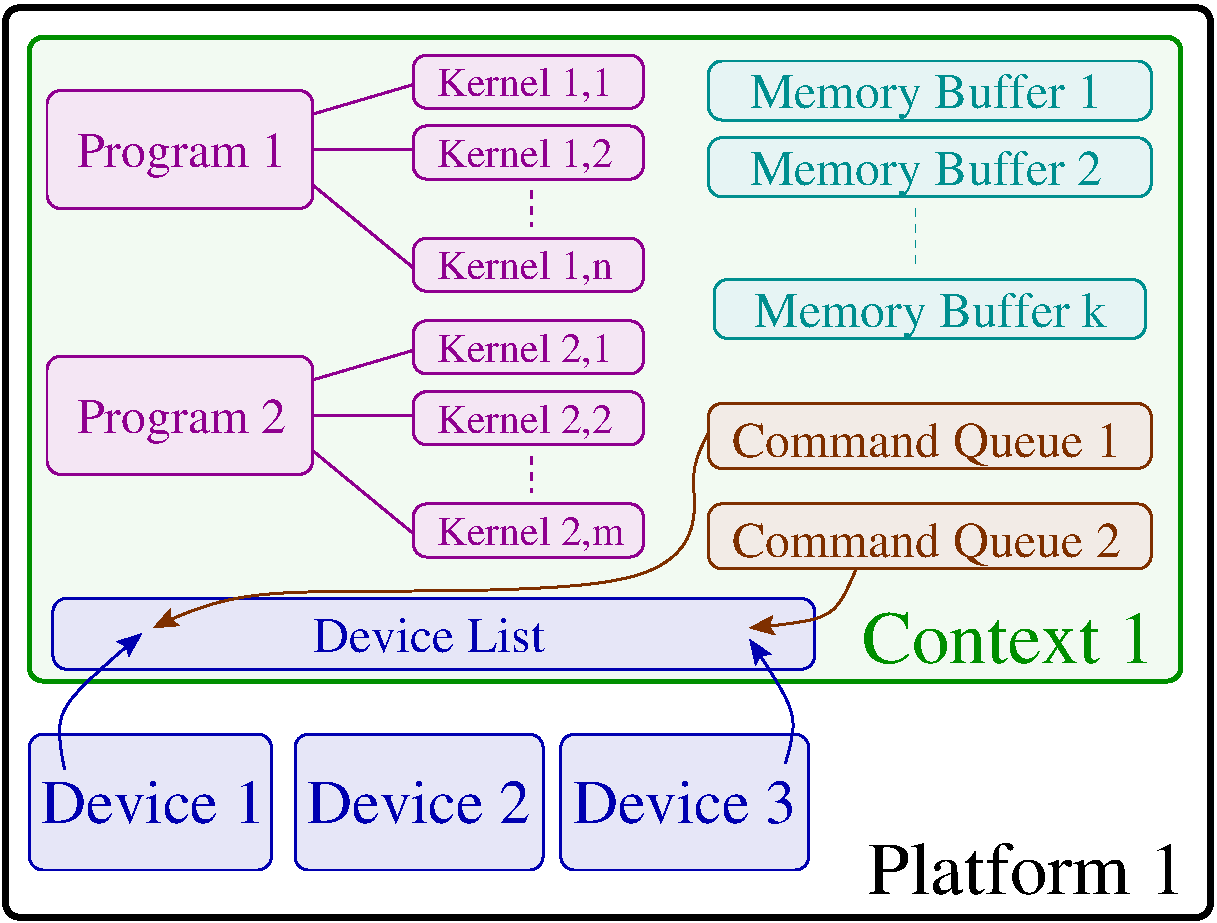
\includegraphics[width=0.80\textwidth]{figures/opencl-full.pdf}
 \end{center}
\end{frame}

\begin{frame}{OpenCL Platform Model}
 \begin{center}
   \Huge https://github.com/karlrupp/phsp2014
 \end{center}
\end{frame}





\begin{frame}[fragile]
\frametitle{OpenCL Host API}

\lstset{ basicstyle=\scriptsize\ttfamily }
\begin{lstlisting}[escapechar=@]
// Setup contet and queue
@\color{red}{context}@ = clCreateContextFromType(NULL, CL_DEVICE_TYPE_GPU, NULL, NULL, NULL);
@\color{red}{queue}@ = clCreateCommandQueue(context, NULL, 0, NULL);

// Create memory buffers
@\color{red}{memobjs[0]}@ = clCreateBuffer(context, CL_MEM_READ_WRITE, sizeof(float)*2*num_entries, NULL, NULL);
@\color{red}{memobjs[1]}@ = clCreateBuffer(context, CL_MEM_READ_ONLY | CL_MEM_COPY_HOST_PTR, sizeof(float)*2*num_entries, srcA, NULL);

// Create OpenCL program and kernels
@\color{red}{program}@ = clCreateProgramWithSource(context, 1, &kernel_src, NULL, NULL);
clBuildProgram(program, 0, NULL, NULL, NULL, NULL);
 
@\color{red}{kernel}@ = clCreateKernel(program, "my_kernel", NULL);
clSetKernelArg(kernel, 0, sizeof(cl_mem), (void *)&memobjs[0]);
clSetKernelArg(kernel, 1, sizeof(cl_mem), (void *)&memobjs[1]);
clSetKernelArg(kernel, 2, sizeof(float)*(local_work_size[0]+1)*16, NULL);
 
// Run an OpenCL kernel:
global_work_size[0] = 128;
 local_work_size[0] = 64;
clEnqueueNDRangeKernel(queue, kernel, 1, NULL, global_work_size, local_work_size, 0, NULL, NULL);
\end{lstlisting}
\lstset{ basicstyle=\small\ttfamily }

\begin{block}{Issues}
 \begin{itemize}
  \item ``Where is the error?''
  \item Manage OpenCL handles
 \end{itemize}

\end{block}

\end{frame}
